\chapter{The Quantum Approximate Optimization Algorithm}
\label{chap:qaoa}

The Quantum Approximate Optimization Algorithm, abbreviated QAOA, was proposed by Farhi, Goldstone and Gutmann in 2014 \cite{FGG14}. The goal of the algorithm is finding approximate solutions to combinatorial optimization problems. Due to its shallow depth it is feasible to run it without error correction on NISQ devides, making it interesting for near-term implementation. The quantum circuit that implements the algorithm prepares a parametrized state, and consists of $p$ layers. Each of the layers comprises of two unitary operators, the first encoding the problem and the latter entangling the qubits, parametrized by some angles. Appropriate parameters can be found in a variety of ways, the most popular being a variational approach similar to the variational quantum eigensolver \cite{VQE}. By sampling from this parametrized state an approximate solution to the problem can be found.
\\

There are two main reasons why QAOA is promising for solving combinatorial optimization problems. First of all because it can be shown that adding extra layers monotonically improves the result of the algorithm. Additionally, in the limit $p \to \infty$, the algorithm produces the optimum, similar to the quantum adiabatic algorithm \cite{FGG14}. Secondly, it is interesting because of its potential to exhibit quantum supremacy \cite{FH16}, as it can not be efficiently simulated by a classical computer. Because of this potential, the algorithm has received quite some attention from the scientific community in the last few years and continues to do so.
\\

In this chapter, I will give an overview of prior work that has been done on QAOA. Specifically, I will explain the general algorithm, how the algorithm can be applied to Max-Cut and how it relates to the Quantum Adiabatic Algorithm that was proposed in \cite{FGGS2000} in 2000. 

\section{General setup}
\label{sec:general-setup}
The Quantum Approximate Optimization Algorithm is designed to handle general optimization problems. These problems can be specified by $n$ bits and $m$ clauses, where a clause is a constraint on a subset of the bits which is satisfied for certain assignments of those bits and not satisfied for other assignments. We want to find a bit string $\vec{x} \in \{0,1\}^n$ of size $n$ that maximizes or minimizes a cost function \cite{FGG14}
\begin{equation}
	C(\vec{x}) \define \sum_{\alpha=1}^m C_\alpha(\vec{x})
	\label{eq:objective}
\end{equation}
where we sum over $m$ clauses that depend on a subset of the $n$ bits. We define $C_\alpha = 1$ if clause $\alpha$ is satisfied and $C_\alpha=0$ otherwise. The goal is to satisfy as many clauses as possible, as that we want to maximize $C(\vec{x})$.
\\
The QAOA is a quantum algorithm that is aimed to find a bit string $\vec{x}'$ for which $C(\vec{x}')$ is close to the maximum of $C$. A quantum computer works in a $2^n$ dimensional vector space, more precisely a Hilbert space in which the norm is induced by an inner product. The computational basis vectors $|\vec{x}\rangle$ can be represented by bit string consisting of $0$s and $1$s. We can consider both the objective function $C$ and the clause $C_\alpha$ in \eqref{eq:objective} as operators that are diagonal in the computational basis.
\begin{equation}
	\hat{C} = \sum_{\vec{x}\in\{0,1\}^n} C(\vec{x})\cdot |\vec{x}\rangle\langle \vec{x} | =  \sum_{\alpha=1}^m \hat{C}_\alpha
	\qquad \text{where} \qquad 
	\hat{C}_\alpha = \sum_{\vec{x}\in\{0,1\}^n} C_\alpha(\vec{x})\cdot |\vec{x}\rangle\langle \vec{x} | = \begin{bmatrix}
	C_\alpha(0, \dots, 0) &  & \\
	& \ddots & \\
	& & C_\alpha(1,\dots, 1)
	\end{bmatrix}
	\label{eq:costHamiltonian}
\end{equation}
We call $\hat{C}$ the \textbf{cost Hamiltonian}. To avoid confusion, I will refer to the operators above as $H_C \equiv \hat{C}$ and $H_{C_\alpha} \equiv \hat{C}_\alpha$ for the rest of this thesis, following the notation from \cite{Hidary}. Using the operator $H_C$, we define the operator $U(H_C, \gamma)$ which depends on some real valued angle $\gamma \in \mathbb{R}$ as follows

\begin{equation}
	U(H_C,\gamma) \define e^{-i\gamma H_C } = \prod_{\alpha = 1}^m e^{-i\gamma H_{C_\alpha}}
	\label{eq:costUnitary}
\end{equation}
I will refer to this object as the \textbf{cost unitary}. Note that the cost Hamiltonian from \eqref{eq:costHamiltonian} is Hermitian, and therefore has purely real eigenvalues, hence the operator $U(H_C,\gamma)$ is indeed unitary. Moreover, observe that the latter equality from \eqref{eq:costUnitary} comes with a caveat. As we want to be able to write $U(H_C, \gamma)$ as a product of local terms it is important that the $H_{C_\alpha}$ commute pairwise. 

\begin{remark}
Remember that the definition of the matrix exponential is derived from the Taylor expansion of the exponent. The exponential of matrix $A$ is given by
\begin{equation}
e^A = \sum_{k=0}^{\infty} \frac{1}{k!}A^k = I + A + \frac{1}{2}A^2 + \frac{1}{6}A^3 + \dots
\end{equation}
Different than taking the exponential of real numbers, the following equality does not always hold for matrix exponents because of possible noncommutativity.
\begin{equation}
e^{A+B} \myeq{?} e^A e^B
\label{eq:matrix-exponential}
\end{equation}
Observe that
\begin{equation}
	e^{A+B} = I + (A+B) + \frac{1}{2}(A+B)^2 + \dots = I + A+B + \frac{1}{2}(A^2 + AB + BA + B^2) + \dots
\end{equation}
\begin{equation}
	e^{A}e^{B} = (I + A + \frac{1}{2}A^2 + \dots)(I + B + \frac{1}{2}B^2 + \dots) = I + A + B + \frac{1}{2}(A^2+2AB+B^2) + \dots
\end{equation}
It can be shown that \eqref{eq:matrix-exponential} only holds if $A$ and $B$ commute, this statement can be extended for arbitrary finite sums. Hence, it is essential for $H_{C_\alpha}$ to commute when separating the cost unitary into local terms in \eqref{eq:costUnitary}.
\end{remark}
If we give every clause equal weight $w_\alpha = 1$, we know that the cost Hamiltonian is diagonal with solely integer entries, which are precisely the eigenvalues of the matrix. We can use the fact that $H_C$ has integer eigenvalues in order to restrict $\gamma$ to be in $[0,2\pi)$. The approach of translating an objective function to an operator is very general and can be applied to a variety of problems. The actual form of $H_C$ is be determined by the specific problem. In section \ref{sec:maxcut-qaoa} I will discuss it in the case of Max-Cut.

Next, we define the operator $H_B$, called the \textbf{mixer Hamiltonian}
\begin{equation}
	H_B \define \sum_{j=1}^n \sigma_x^{(j)}
	\label{eq:mixerHam}
\end{equation}
where $\sigma_x^{(j)}$ is the Pauli-$X$ gate acting solely on the qubit $j$.
\begin{equation}
	\sigma_x^{(j)} = I^{\otimes j-1} \otimes \sigma_x \otimes I^{\otimes n-j}
\end{equation}
where $I$ is the $2\times 2$ identity matrix, $\otimes$ denotes the Kronecker product and $A^{\otimes n}$ denotes the Kronecker product of a matrix $A$ with itself $n$ times. 
\begin{equation}
	A^{\otimes n} = \underbrace{A \otimes \dots \otimes A}_{n \text{ times}}
\end{equation}

Using the mixer Hamiltonian, we can define another unitary operator, the \textbf{mixer unitary}, similar to what we did before
\begin{equation}
	U(H_B,\beta) \define e^{-i\beta H_B} = \prod_{j=1}^n e^{-i \beta \sigma_x^{(j)}}
	\label{eq:mixerUnitary}
\end{equation}

where again $\beta \in \mathbb{R}$ is some real angle. Note that $\sigma_x^{(j)}$ commute pairwise so when taking the exponential of $H_B$ that is the sum of these terms, expression \eqref{eq:matrix-exponential} holds and we are able to construct $H_B$ with local gates. With these unitaries defined, we can move on to the next part: preparing the parameterized state. We start of in the initial equal superposition state
\begin{equation}
	|s\rangle \define \frac{1}{\sqrt{2^n}}\sum_{x\in \{0,1\}^n} |x \rangle = |+\rangle^{\otimes n} = H^{\otimes n}|0\rangle^{\otimes n}
\end{equation} 
which is easy to prepare using Hadamard gates applied to each of the $n$ qubits, all in the state $|0\rangle$. 
Thereafter, we alternately apply the cost Hamiltonian and the mixer Hamiltonian $p$ times, using different parameters $\gamma_1 \dots \gamma_p$ and $\beta_1 \dots \beta_p$, respectively. 
\begin{equation}
	|\vec{\gamma}, \vec{\beta}\rangle \define \underbrace{ U(H_B,\beta_p)U(H_C,\gamma_p) \dots \underbrace{U(H_B,\beta_1)U(H_C,\gamma_1)}_{\text{one layer}}}_{p \text{ layers}}|s\rangle
\end{equation}
I use boldface vector notation $\gambe$ for the sole purpose of writing these sets of parameters more compactly. Furthermore, take note that we work from right to left, as is convention when working with matrices. See Figure \ref{fig:schematic-qaoa} for a schematic of the circuit preparing the parametrized state. Now that we have established this, we can move on to the actual aim of this circuit. The idea is to find parameters such that 
\begin{equation}
	F_p(\gambe) \define \langle \gambe |H_C| \gambe \rangle
\end{equation}
is maximized, where we indicate the number of layers $p$ using a subscript. In general, $\vec{\gamma},\vec{\beta} \in \mathbb{R}^p$, however depending on the cost and mixer unitaries we can restrict the domain using symmetries. We define 
\begin{equation}
M_p \define \max_{\gambe} F_p(\gambe)
\end{equation} and want to find the corresponding parameters. By sampling from this state $|\gambe \rangle$ we can find an approximate solution by looking at either the most sampled bit string, or the best sampled bit string.

The reader might wonder why we need to apply the mixer unitary when only the cost unitary encodes the problem. This has to do with the way probabilities work in quantum mechanics. The probability of measuring a bit string that encodes a particular solution, is precisely the square magnitude of the corresponding amplitude. Take note of the fact that the exponent of a diagonal $n \times n$ matrix $A = \diag{a_{11}, \dots a_{nn}}$ is a diagonal matrix with the entries exponentiated.  
\begin{equation}
	e^{\diag{a_{11},\dots a_{nn}}} = \diag{e^{a_{11}},\dots, e^{a_{nn}}}
\end{equation}

Since the cost Hamiltonian $H_C$ is diagonal and real, the cost unitary will be diagonal with entries of the form $e^{i\phi}$ for some $\phi \in \mathbb{R}$. This implies that the amplitudes will only acquire relative phases, and thus the probability of finding a particular bit string is not affected by the cost unitary. If we were going to run a circuit with only cost unitaries, it would result in an equal superposition, whatever set of angles $\vec{\gamma}$ we choose. A fancy way of implementing the random partition algorithm from Section \ref{sec:random-partition}. For this reason we need an operator that entangles the states to do better than the random partition algorithm, hence the need for the mixer Hamiltonian.

Finding the optimal, or even a good set of angles $\gambe$ is a non-trivial task. In Section \ref{sec:optimal-parameters} a more thorough discussion on this topic can be found. Furthermore, one method for finding the angles proposed in \cite{ZWCPL18}, called INTERP, is discussed in more depth in Chapter \ref{chap:implementation}, which will also be used to produce the results in Chapter \ref{chap:results}.

\begin{figure}[H]
	\centering
	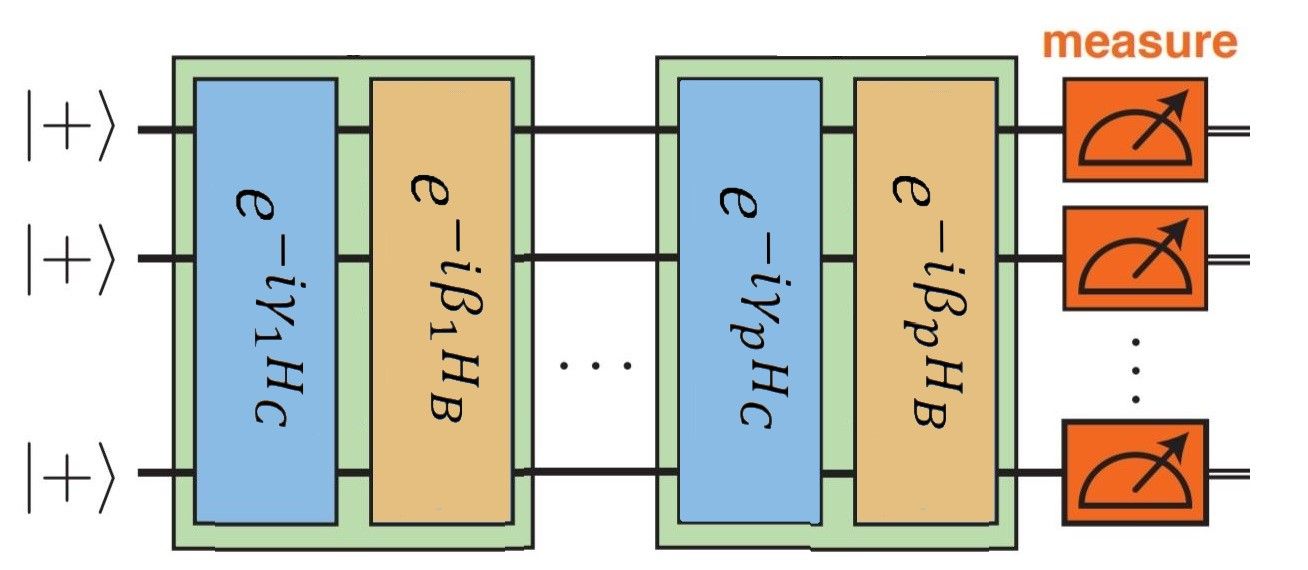
\includegraphics[width=0.8\textwidth]{figures/qaoa_idea_edit.JPG}
	\caption{Schematic of a $p$-level Quantum Approximation Optimization Algorithm. The cost unitary and the mixer unitary are alternately applied to prepare the parametrized state $|\gambe\rangle$. Adapted figure from \cite{ZWCPL18}.}
	\label{fig:schematic-qaoa}
\end{figure}

\section{Applying QAOA to Max-Cut}
\label{sec:maxcut-qaoa}
QAOA can easily be applied to the Max-Cut problem by associating each vertex $i \in V$ with a qubit $q_i$ and using the qubit's state to encode the affiliation to one of the sets of the bipartition. A qubit in state $|1\rangle$ means it is in one half of the bipartition, $S$, a qubit in state $|0\rangle$ means it is in the other, namely $\bar{S}$. Our aim is to find a cut such that we maximize the sum of the edges in the cut, so we would like adjacent qubits to be in different halves of the bipartition. As explained in Section \ref{section:maxcut}, we can express this mathematically as
\begin{equation}
	C(\vec{z}) = \frac{1}{2}\sum_{\{i,j\}\in E} w_{i,j}(1-z_i z_j)
\end{equation}
where $z_i \in \{-1,1\}$ for $i\in V$. Now the idea is to translate this problem into a cost Hamiltonian. Remark that the Pauli matrix $\sigma_z = \diag{1,-1}$ has eigenvalues $1$ and $-1$. Therefore, we can use $\sigma_z^{(i)}$ to represent $z_i$. Using this we can define the cost Hamiltonian to be
\begin{equation}
	H_C = \frac{1}{2} \sum_{\{i,j\}\in E} w_{i,j}\big(I-\sigma_z^{(i)}\sigma_z^{(j)}\big)
\end{equation}
Note that the term $I-\sigma_z^{(i)}\sigma_z^{(j)}$ involving qubits $i$ and $j$ is diagonal in the computational basis. This is important because we want to be able to write the cost unitary as a product of local terms
\begin{equation}
	U(H_C, \gamma) = e^{-i\gamma H_C} = \prod_{\alpha=1}^m e^{-\gamma H_{C_\alpha}} = \prod_{\{i,j\}\in E} e^{-\gamma \frac{w_{i,j}}{2}\big(I-\sigma_z^{i}\sigma_z^{j}\big)}
\end{equation}
Since all the terms in the product are diagonal, they all commute as desired. Now we have all the ingredients to prepare the state $|\gambe\rangle$ for Max-Cut using the unitary operators $U(H_C, \gamma)$ and $U(H_B, \beta)$. 

The actual outcome of the algorithm is determined by sampling from the state $|\gambe\rangle$ and calculating the cut value corresponding to the measured bit string on a classical computer. This yields a distribution of bit strings (and cutvalues). However, in the end we want one solution and not a distribution. One option would be to pick the most sampled bit string, but performance is easily improved by picking the best sampled bit string instead.

Now, we only need to find out how to implement this in a circuit and figure out a way for finding appropriate angles $\gambe$. This will be discussed in Subsection \ref{subsec:circuit} and Section \ref{sec:optimal-parameters}, respectively.

\subsection{Quantum circuit design}
\label{subsec:circuit}
It is useful to know about the rotation operators $R_x$ and $R_z$ when wanting to implement the unitary operators $U(H_C,\gamma), U(H_B,\beta)$. These operators induce rotations around their respective axes, and are defined as follows
\begin{equation}
		R_x(\theta) \equiv e^{-\frac{\theta i}{2} \sigma_x} = \begin{bmatrix}
			\cos(\theta/2) & -i\sin(\theta/2) \\
			-i\sin(\theta/2) & \cos(\theta/2)
		\end{bmatrix}
\end{equation}
\begin{equation}
	R_z(\theta) \equiv e^{-i\frac{\theta}{2} \sigma_z} = \begin{bmatrix}
	e^{-i \theta /2} & 0 \\
		0 & e^{i\theta/2}
	\end{bmatrix}
\end{equation}
Furthermore, we need a $\CNOT$ gate \cite{Mike&Ike}, which involves 2 qubits
\begin{equation}
	\CNOT_{q_i,q_j} = |0\rangle \langle0| \otimes I + |1\rangle \langle1|\otimes X  = \begin{bmatrix}
	1 & 0 & 0 & 0 \\
	0 & 1 & 0 & 0 \\
	0 & 0 & 0 & 1 \\
	0 & 0 & 1 & 0 \\
	\end{bmatrix} 
	= 
	\Qcircuit @C=1em @R=.7em {
		&q_i& & \ctrl{1} & \qw  \\
		&q_j& & \targ  & \qw \\
	}
\end{equation}
To understand this component intuitively, the target qubit $q_j$ will be flipped if the control qubit $q_i$ is $1$. As we are working with qubits, this does not encapsulate the complete picture, so we need to describe it with a matrix instead. 

The $X$-interactions in the mixer Hamiltonian can be implemented with this one-qubit gate $R_x$.
\begin{equation}
	e^{-i\beta\sigma_x^{(i)}} \equiv \Qcircuit @C=1em @R=.7em {
		&q_i& & \gate{R_x(2\beta)}  & \qw\\
	}
\end{equation}
The two-qubit $ZZ$-interactions in the cost unitary can be implemented with two $\CNOT$ gates, and the local one-qubit gate $R_z$ \cite{Crooks18}. Since $\sigma_z^{(i)}$ and $\sigma_z^{(j)}$ commute the roles of $q_i$ and $q_j$ are interchangable.
\begin{equation}
e^{-\frac{i}{2}\gamma(I-\sigma_z^{(i)}\sigma_z^{(j)})} \equiv \Qcircuit @C=1em @R=.7em {
	&q_i& & \ctrl{1} & \qw & \ctrl{1}  & \qw \\
	&q_j& & \targ \qw & \gate{R_z(-\gamma)} & \targ & \qw\\
} 
\equiv 
\Qcircuit @C=1em @R=.7em {
	&q_i& & \targ \qw & \gate{R_z(-\gamma)} & \targ & \qw\\
	&q_j& & \ctrl{-1} & \qw & \ctrl{-1}  & \qw \\
} 
\end{equation}

As both $U(H_C,\gamma)$ and $U(H_B,\beta)$ are both products of local terms, we only need those terms to implement them. The final circuit first applies Hadamards to each qubit in order to create an equal superposition over all bit strings, or possible partitions if you will. Next we apply the cost unitary and the mixer unitary in an alternating fashion, in that order, with desired angles. Lastly, we measure the state to get an actual bit string.

As an example, consider the unweighted \emph{diamond graph}, visualised in Figure \ref{fig:graph-diamond}. 

\begin{figure}[H]
	\centering
	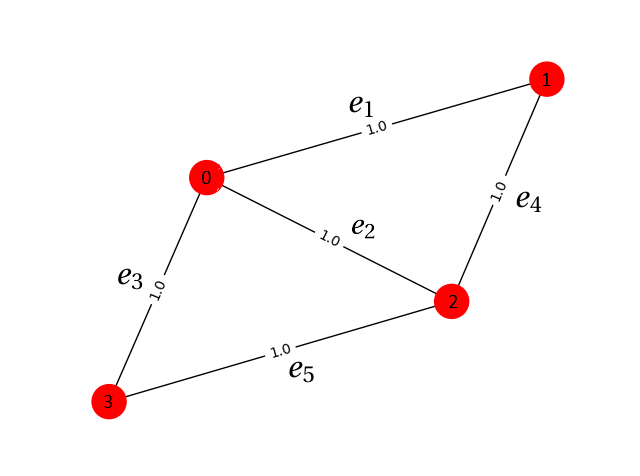
\includegraphics[width=0.35\textwidth]{figures/diamond-graph-edges}
	\caption{Diamond graph (unweighted)}
	\label{fig:graph-diamond}
\end{figure}

The graph consists of 4 nodes, whereof 2 nodes connect to 2 edges, and 2 nodes connect to 3 edges. The circuit needed to prepare the state $|\gamma,\beta \rangle$ with $p=1$ for this particular graph is given in Figure \ref{fig:circuit}.
In general, the depth of the circuit, assuming no overhead necessary for swapping is then at most $p(3m+n)$ where $p$ is the number of QAOA layers, $n$ is the number of nodes, or qubits and $m$ is the number of edges in the graph. For a graph with $n$ nodes we can bound $m$ by $\frac{1}{2}n(n-1)$, the number of edges in a complete graph. Concluding, we see that the circuit requires $O(n^2)$ gates assuming full qubit connectivity. %In actual hardware one usually encounters qubits arranged in a 2-dimensional lattice with gates only between nearest neighbours. Hence, SWAP gates are necessary to move logical qubits into proximity. It turns out that QAOA can be efficiently implemented with $O(n)$ overhead \cite{Crooks18}.  \hl{elab on swaps}

\begin{figure}[H]
	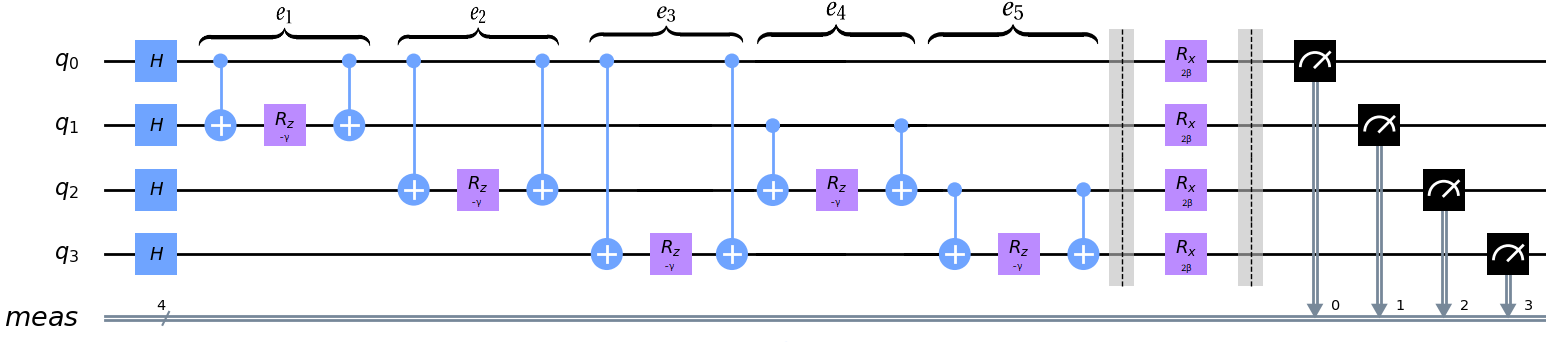
\includegraphics[width=\textwidth]{figures/circuit_diamond_edit2.png}
	\caption{Circuit for the diamond graph from Figure \ref{fig:graph-diamond} with parameters $\gamma$ and $\beta$ for the rotations using the cost and mixer Hamiltonians respectively. Every node in the graph is represented by a qubit, and the cost unitary can be implemented with two CNOT gates with a $R_z(-\gamma)$ gate in between for every edge in the graph, the relation to the graph edges is indicated with the braces. After the cost unitary, the mixer unitary is applied. This operator can be broken down into rotation gates $R_x(2\beta)$ applied to every qubit, or node. Finally, the system is measured in the computational basis.}
	\label{fig:circuit}
\end{figure}

\subsection{Maximizing the expectation value}
To give a sense of what it means to improve the expectation value of the cost function, several barplots are shown of the distribution resulting from sampling from three different states $|\gambe\rangle_{(p)}$ for $p=1,2,3$ after optimizing the angles for the diamond graph. As we can see, as we increase $p$ we are able to improve the expecation value and get good bit strings with high probability. In Section \ref{sec:optimal-parameters} I will go into more depth on how to determine an appropriate set of angles.

\begin{figure}[H]
	\centering
	\begin{subfigure}[t]{0.62\textwidth}
		\centering
		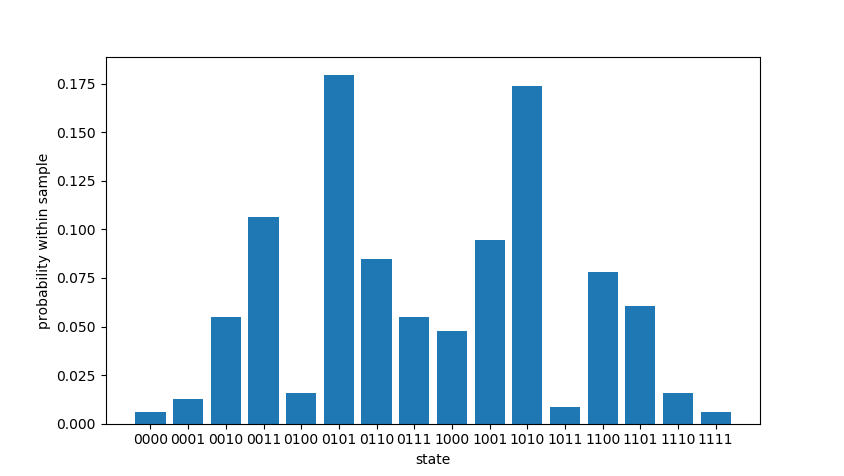
\includegraphics[width=\textwidth]{figures/histogram/diamond_p1.png}
		\captionsetup{justification=centering}
		\caption{$p=1$}
	\end{subfigure}
	\\
	\centering
	\begin{subfigure}[t]{0.62\textwidth}
		\centering
		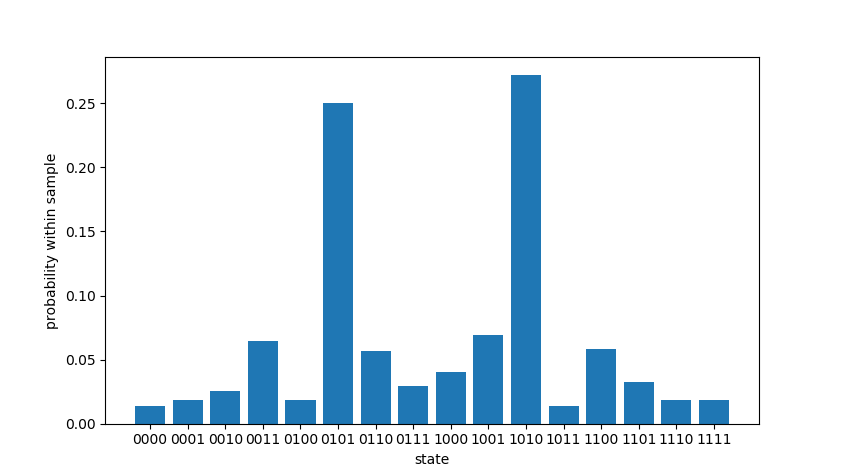
\includegraphics[width=\textwidth]{figures/histogram/diamond_p2.png}
		\captionsetup{justification=centering}
		\caption{$p=2$}
	\end{subfigure}
	\\
	\centering
	\begin{subfigure}[t]{0.62\textwidth}
		\centering
		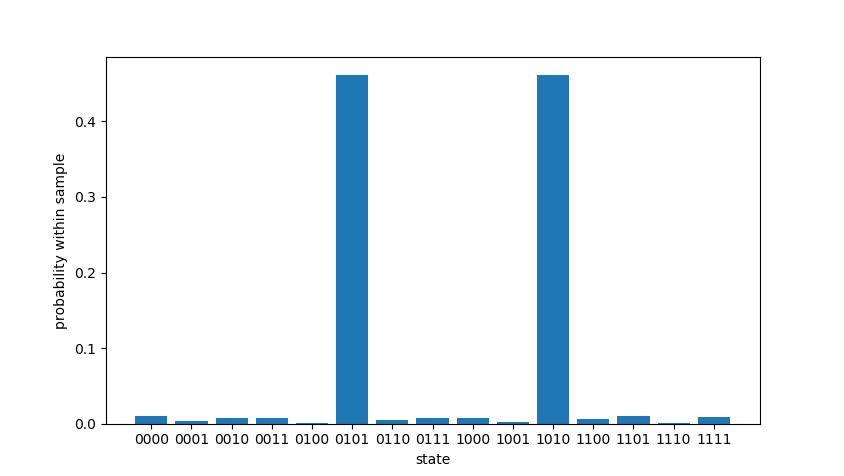
\includegraphics[width=\textwidth]{figures/histogram/diamond_p3.png}
		\captionsetup{justification=centering}
		\caption{$p=3$}
	\end{subfigure}
	\caption{Histograms of the distribution when sampling from the state $|\gambe\rangle_{(p)}$ for $p=1,2,3$ with $\vec{\gamma},\vec{\beta} \in \mathbb{R}^p$. The three sets of parameters are determined using BFGS optimization starting with a randomly chosen intial point. For these angles we have $F_1 = 3.24$, $F_2 = 3.39$, $F_3 = 3.87$. The order of the bits is $(0,1,2,3)$ where the labelling of the nodes is the same as in Figure \ref{fig:graph-diamond}. The optimal partitions are 0101 and 1010 with cutvalue 4.}
\end{figure}

\newpage

\subsection{Expectation landscapes}
To provide insight to what kind of expectation landscapes we might encounter, I will discuss the relevant features and symmetries that come into play in this section. In addition, I will show some expectation landscapes in the case of $p=1$.

For unweigthed graphs we find periodicity in the $\gamma$ direction. As mentioned in Section \ref{sec:general-setup}, this has to do with the fact that the cost Hamiltonian $H_C$ has integer eigenvalues, resulting in the identity
\begin{equation}
e^{2\pi i H_C} = I
\end{equation}
yielding a period of $2\pi$ in the $\gamma$ parameter in all layers. Moreover, there is $\mathbb{Z}_2$ symmetry to be exploited. This means that the partition $(S,\bar{S})$ is equivalent to the partition $(\bar{S},S)$, or in terms of bit strings a partition $10101$ is equivalent to $01010$ as the inversed labelling does not alter the value of a cut. Therefore if we apply $X^{\otimes n}$ to the state $|\gambe\rangle$ it does not change the expectation value $F_p = \langle H_C \rangle$. Note that the mixer unitary can be constructed with $R_x(2\beta)$ gates, but since $R_x(2\pi) \hat{=} X$ (up to global phase) we find a periodicity of $\pi$ in the $\beta$ parameter. Hence we can restrict $\beta \in [0,\pi)$ in general. Concluding, for unweighted graphs we have
\begin{equation}
\langle \gambe |H_C | \gambe \rangle = \langle \vec{\gamma} + 2\pi \vec{n}, \vec{\beta} + \pi\vec{m}|H_C|\vec{\gamma} + 2\pi \vec{n}, \vec{\beta} + \pi\vec{m}\rangle \qquad \vec{n},\vec{m} \in \mathbb{N}^p
\end{equation}
and for weighted graphs we have
\begin{equation}
\langle \gambe |H_C | \gambe \rangle = \langle \vec{\gamma}, \vec{\beta} + \pi\vec{m}|H_C|\vec{\gamma}, \vec{\beta} + \pi\vec{m}\rangle \qquad \vec{m} \in \mathbb{N}^p
\end{equation}

In Figures \ref{fig:landscapes-diamond} and \ref{fig:landscapes-butterfly} some examples of $F_1$ landscapes are shown. Remember that $F_1 = \langle \gamma, \beta | H_C | \gamma, \beta \rangle$ was defined to be the expectation value of the cost Hamiltonian. This means that if we repeatedly prepare the state $|\gamma,\beta\rangle$ and calculate the cut values, the average will be $F_1(\gamma,\beta)$. As explained, the aim is to seek values for $\gamma, \beta$ that maximize this quantity.
\begin{figure}[H]
	\begin{subfigure}[t]{0.42\textwidth}
		\centering
		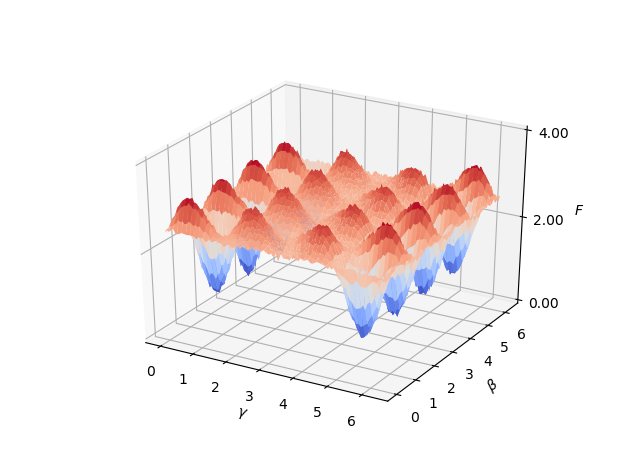
\includegraphics[width=\textwidth]{figures/landscape_new/diamond_3D.png}
		\caption{3D plot of $F_1$ for the unweighted diamond graph}
		\label{subfig:Diamond3D}
	\end{subfigure}%
	~ 
	\begin{subfigure}[t]{0.42\textwidth}
		\centering
		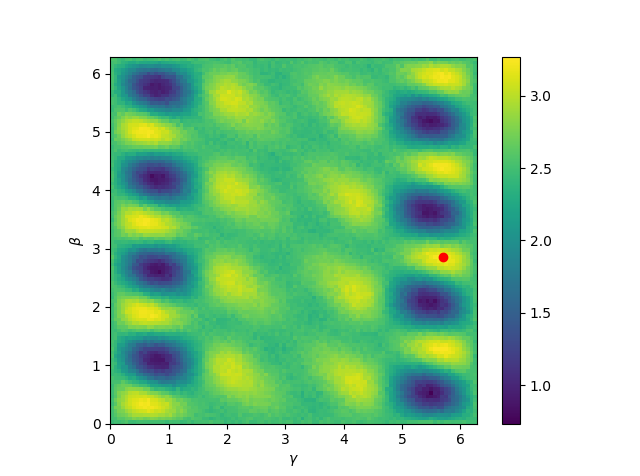
\includegraphics[width=\textwidth]{figures/landscape_new/diamond_imshow.png}
		\caption{Colorplot of $F_1$ for the unweighted diamond graph}
	\end{subfigure}
	\\
	\centering
	\begin{subfigure}[t]{0.45\textwidth}
		\centering
		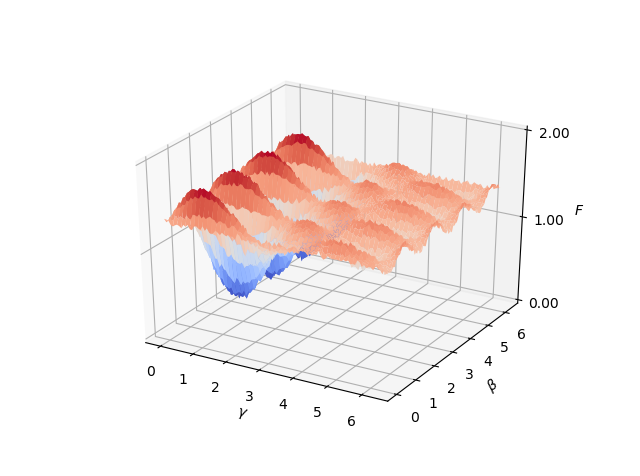
\includegraphics[width=\textwidth]{figures/landscape_new/diamond_weighted_3D.png}
		\caption{3D plot of $F_1$ for the weighted diamond graph.}
	\end{subfigure}%
	~ 
	\begin{subfigure}[t]{0.45\textwidth}
		\centering
		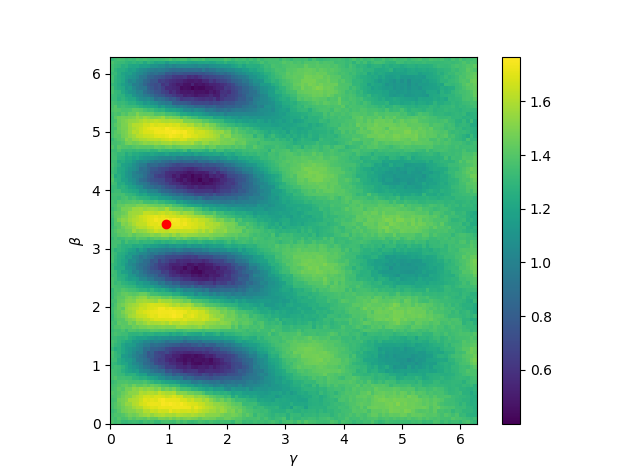
\includegraphics[width=\textwidth]{figures/landscape_new/diamond_weighted_imshow.png}
		\caption{Colorplot of $F_1$ for the weighted diamond graph}
	\end{subfigure}
	\caption{Landscapes of the expectation value $F_1$ for the unweighted (a), (b) and weighted (c), (d) Diamond graph (Figure \ref{fig:graph-diamond}) using a 3D plot and a colorplot respectively. The weights for the weighted graph were drawn from a uniform distribution $w_{ij} \sim U(0,1)$ for the weights of edges $\{i,j\} \in E$. In all plots both $\gamma, \beta$ range from $0$ to $2\pi$, divided into $100$ gridpoints. The expectation value $F_1 = \langle H_C\rangle$ is estimated using 1024 samples from the state $|\gamma, \beta \rangle$ at each gridpoint. The maximum is indicated by a red dot in the colorplots, note however that due to symmetries the actual optima are degenerate.}
	\label{fig:landscapes-diamond}
\end{figure}

\newpage
\begin{figure}[H]
	\centering
	\begin{subfigure}[t]{0.6\textwidth}
		\centering
		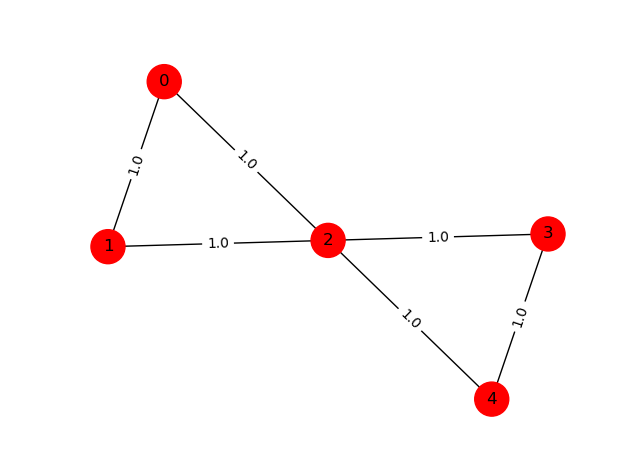
\includegraphics[width=\textwidth]{figures/butterfly-graph.png}
		\caption{Butterfly graph (unweighted)}
	\end{subfigure}%
	\\
	\centering
	\begin{subfigure}[t]{0.5\textwidth}
		\centering
		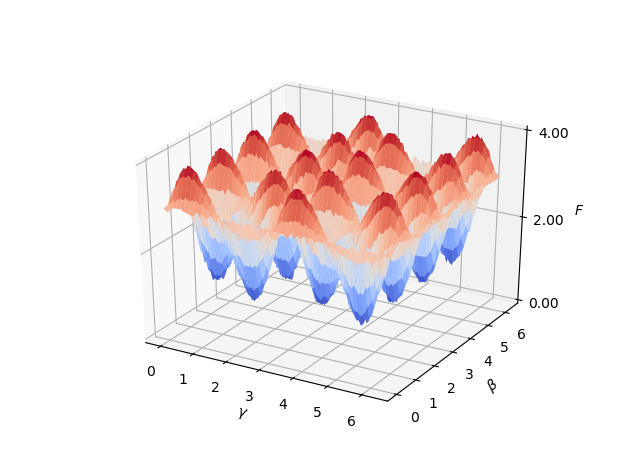
\includegraphics[width=\textwidth]{figures/landscape_new/butterfly_3D.png}
		\caption{3D plot of $F_1$ for the butterfly graph}
	\end{subfigure}%
	~ 
	\begin{subfigure}[t]{0.5\textwidth}
		\centering
		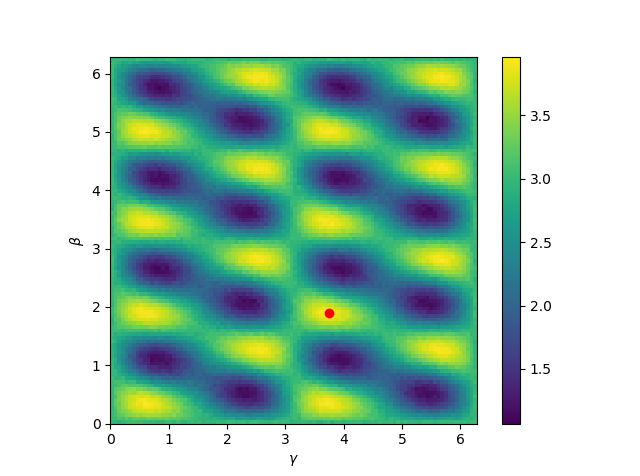
\includegraphics[width=\textwidth]{figures/landscape_new/butterfly_imshow.png}
		\caption{Colorplot of $F_1$ for the butterfly graph}
	\end{subfigure}
	\\
	\centering
	\begin{subfigure}[t]{0.5\textwidth}
	\centering
	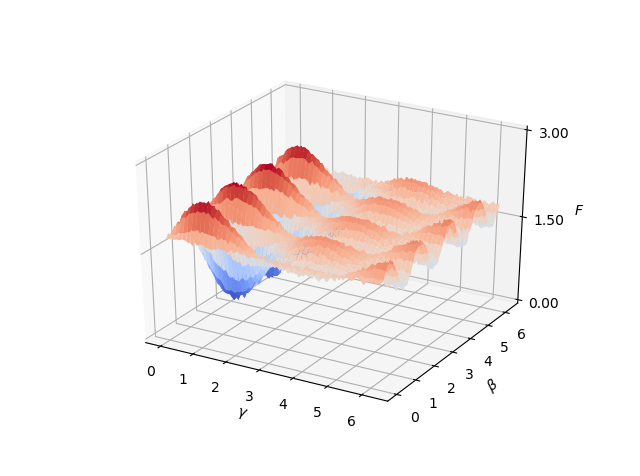
\includegraphics[width=\textwidth]{figures/landscape_new/butterfly_weighted_3D.png}
	\caption{3D plot of $F_1$ for the weighted butterfly graph}
	\end{subfigure}%
	~ 
	\begin{subfigure}[t]{0.5\textwidth}
	\centering
	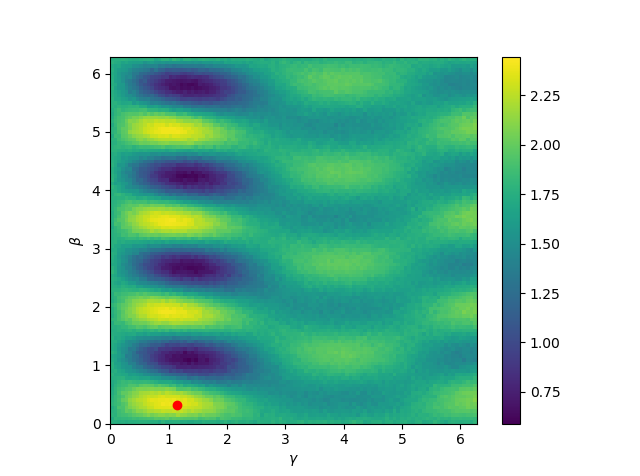
\includegraphics[width=\textwidth]{figures/landscape_new/butterfly_weighted_imshow.png}
	\caption{Colorplot of $F_1$ for the weighted butterfly graph}
	\end{subfigure}
	\caption{Landscapes of the expectation value $F_1$ for the unweighted (b), (c) and weighted (d), (e) Butterfly graph using a 3D plot and a colorplot respectively. The graph is visualized in (a). The weights for the weighted graph were drawn from a uniform distribution $w_{ij} \sim U(0,1)$ for the weights of edges $\{i,j\} \in E$. In all plots both $\gamma, \beta$ range from $0$ to $2\pi$, divided into $100$ gridpoints. The expectation value $F_1 = \langle H_C\rangle$ is estimated using 1024 samples from the state $|\gamma, \beta \rangle$ at each gridpoint. The maximum is indicated by a red dot in the colorplots, note however that due to symmetries the actual optima are degenerate.}
	\label{fig:landscapes-butterfly}
\end{figure}

\subsection{Adiabatic Theorem and the limit $p \to \infty$}
\label{subsec:adiabatic-theorem}
One of the main advantages of QAOA is the fact that its performance monotonically increases with $p$. This can be shown using the Adiabatic Theorem.
\begin{theorem}
	Suppose that the Hamiltonian of a system gradually changes from an initial form $H_i$ to some final form $H_f$. The Adiabatic Theorem states that if the system was initially in the $n$th eigenstate of $H_i$, then at the end of the process, the system will be in the $n$th eigenstate of $H_f$ \cite{Griffiths}. 
\end{theorem}

I would like to emphasize that this change has to be gradual, hence the name adiabatic (very much related to the same term in the context of thermodynamics). Using the Adiabatic Theorem it can be proven that as $p\to \infty$ the QAOA obtains the optimimal solution \cite{FGG14}
\begin{equation}
\lim_{p\to \infty} \max_{\gambe} F_p(\gambe) = \max_{\vec{x}} C(\vec{x})
\end{equation}
This configuration $\vec{x}$ corresponds to the is the groundstate energy of $-H_C$, where $H_C$ is the cost Hamiltonian defined in \eqref{eq:costHamiltonian}.

\subsection{Concentration}
\label{subsec:concentration}
While it is useful that we are guaranteed to improve the expectation ratio $F_p$ when increasing $p$, eventually we want to sample from the state $|\gambe\rangle$ to find an approximate solution. For this reason, it is desirable to know if the variance is bounded or not, since we would like to find bit strings with a cutvalue close to $F_p$ or better. This turns out to be the case. In the original paper \cite{FGG14}, it was proven that the variance is bounded by the following quantity.
\begin{equation}
\langle \vec{\gamma},\vec{\beta}|C^2|\vec{\gamma},\vec{\beta}\rangle - \langle \vec{\gamma},\vec{\beta}|C|\vec{\gamma},\vec{\beta}\rangle^2 \leq 2m \bigg[\frac{(v-1)^{2p+2}-1}{(v-1)-1}\bigg]
\label{eq:concentration}
\end{equation}
where $v$ is the maximum degree of the graph and $m$ the number of edges (or clauses). When $v$ and $p$ are taken to be constant, the standard deviation of $C(z)$ is at most of order $\sqrt{m}$. This has the advantageous implication that the sample mean of order $m^2$ values of $C(z)$ satisfies $|F_p(\vec{\gamma},\vec{\beta}) - C(z)| \leq 1$ with probability $1-\frac{1}{m}$, as we can estimate $F_p(\vec{\gamma},\vec{\beta})$ with a reasonable amount of samples.

\section{Finding optimal parameters}
\label{sec:optimal-parameters}
Several methods for finding optimal angles have been proposed in \cite{BBFGH18, Crooks18, ZWCPL18}. These methods include solving the problem analytically, doing a gridsearch of the parameter space \cite{FGG14}, using known optimization methods such as Nelder-Mead \cite{VBB17} or the Broyden–Fletcher–Goldfarb–Shanno algorithm \cite{ZWCPL18}, and even machine learning \cite{Crooks18, AAG20}. 

The first two approaches unfortunately do not scale well with $p$. Analytically solving for the optimal parameters requires evaluation of subgraphs of depth $p$. On the other hand, one could use a gridsearch by dividing the parameter space into $N$ points. This approach seems promising for fixed $p$, as the $F$-landscape is usually not jagged. To be precise, the partial derivatives of $F_p(\gambe)$ were shown to be bounded by $O(m^2+mn)$ \cite{FGG14}. There is one downside to this, to determine $2p$ parameters, we would have to estimate the expectation of the cost function $N^{2p}$ times, as this method is not at all efficient in $p$. There are also methods that use a variational approach, as will be discussed in the next section.

\subsection{Variational Quantum Eigensolver}
\label{sec:vqe}
The variational quantum eigensolver (VQE) is a quantum algorithm used to find the groundstate of a given Hamiltonian $H$ \cite{VQE, MRBA16}. It makes use of the variational principle which states that the expectation value of the Hamiltonian is always greater than or equal to the groundstate energy $E_0$  \cite{Griffiths}
\begin{equation}
\langle H \rangle \geq E_0
\end{equation}
for any state $|\psi\rangle$. The idea of VQE is to prepare a parameterized state $|\psi  (\vec{\theta}) \rangle$ that depends on some parameter set $\vec{\theta}$. This state is prepared using a unitary operator $U(\vec{\theta})$.
\begin{equation}
|\psi (\vec{\theta}) \rangle = U(\vec{\theta})|0\rangle
\label{eq:vqe-parametrized-unitary}
\end{equation} 
Using the variational principle, the ground state energy can be bound by $\langle \psi(\vec{\theta})|H|\psi(\vec{\theta})\rangle$. The actual goal is to find the optimal set $\vec{\theta}$ in order to prepare the groundstate, or a state that is close to it
\begin{equation}
\vec{\theta}_{\text{opt}} = \arg \min_{\vec{\theta}} \langle \psi(\vec{\theta})|H|\psi(\vec{\theta})\rangle
\end{equation}
The optimal parameters can be found with outer-loop classical optimization, see Figure \ref{fig:vqe}. Examples of possible methods include Nelder-Mead \cite{NelderMead}, the Broyden–Fletcher–Goldfarb–Shanno (BFGS) algorithm \cite{BFGS} or particle swarm optimization \cite{PSO1, PSO2}.

\begin{figure}[H]
	\centering
	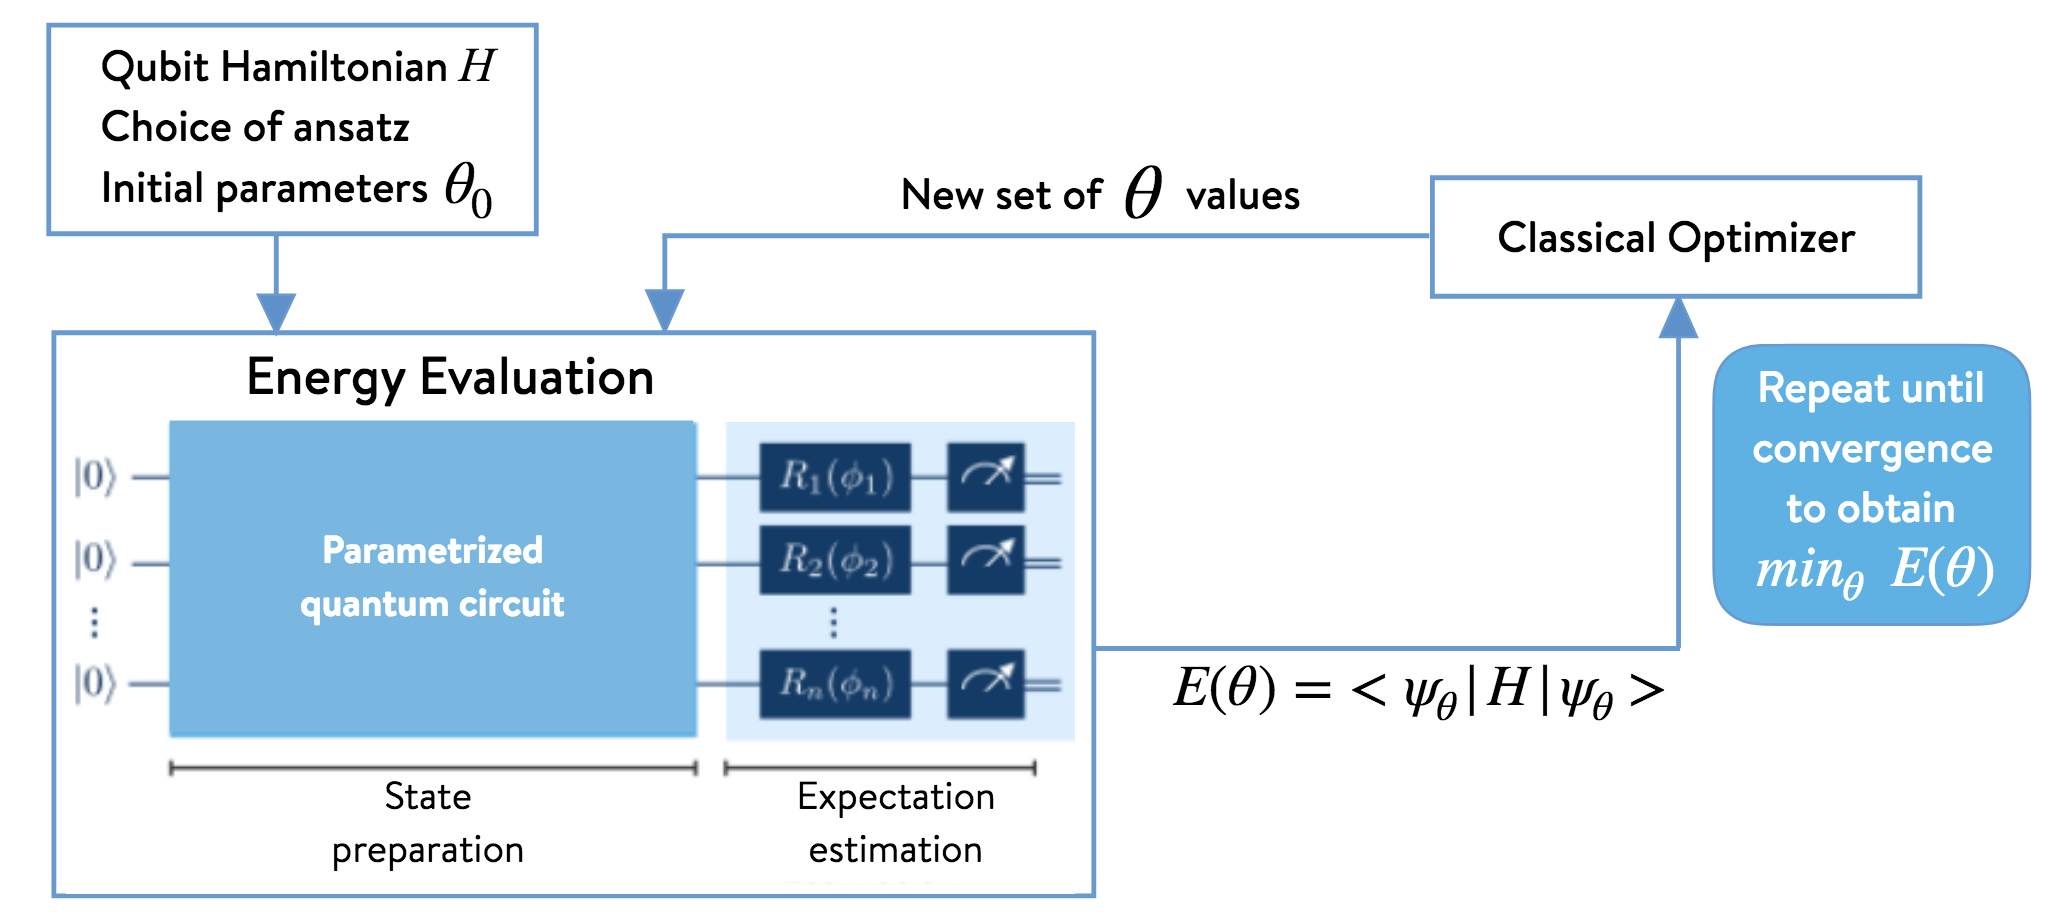
\includegraphics[scale=0.4]{figures/VQE_overview.png}
	\caption{Overview of the variational quantum eigensolver. A parametrized state is prepared after which the expectation value of the Hamiltonian is calculated classically. A classical optimization scheme determines a new set of parameters to be tried. This is repeated until convergence, or some other stopping criterium. Figure from \cite{vqe-figure}}
	\label{fig:vqe}
\end{figure}

It should be noted that the set of states that are possible to create is restricted by the structure of $U(\vec{\theta})$. Finding an appropriate ansatz operator $U(\vec{\theta})$ necessary to find the true groundstate can be difficult without prior knowledge of the problem.

Note that this is very similar to what we have to do in QAOA, namely finding the set of parameters $\gambe$ to maximize the expectation value of the cost Hamiltonian $H_C$, which is equivalent to minimizing the expectation value of $-H_C$
\begin{equation}
\vec{\gamma}_{\text{opt}}, \vec{\beta}_{\text{opt}} = \arg \min_{\vec{\gamma}, \vec{\beta}} \langle \gambe | -H_C | \gambe \rangle
\end{equation}
The form of the unitary in \eqref{eq:vqe-parametrized-unitary} in the case of QAOA is given by
\begin{equation}
	U(\vec{\gamma}, \vec{\beta}) = U(\beta_p, H_B)U(\gamma_p, H_C) \dots U(\beta_1, H_B)U(\gamma_1, H_C)H^{\otimes n}
\end{equation}

In fact, we can use VQE as a subroutine of QAOA for finding the optimal parameters \cite{ZWCPL18, Yao20}. An illustration hereof can be found in Figure \ref{fig:schematic-qaoa-vqe}. VQE is still an active field of research \cite{active-1,active-2,active-3}. It can be applied to QAOA, but also to areas such as chemistry where it is used for finding the groundstate energy of simple molecules \cite{VQE}.

In this thesis I will investigate one of the methods proposed in \cite{ZWCPL18} that makes use of the VQE subroutine. This method exploits certain patterns relating the optimal angles for different layers of the algorithm, reminiscent of the Quantum Adiabatic Algorithm. These patterns can be used to iteratively increase $p$, and determining an educated guess for the next QAOA layer from which an optimization routine is started for finding the local optimum. A more in depth discussion of these methods can be found in chapter \ref{chap:implementation}.
\begin{figure}[H]
	\centering
	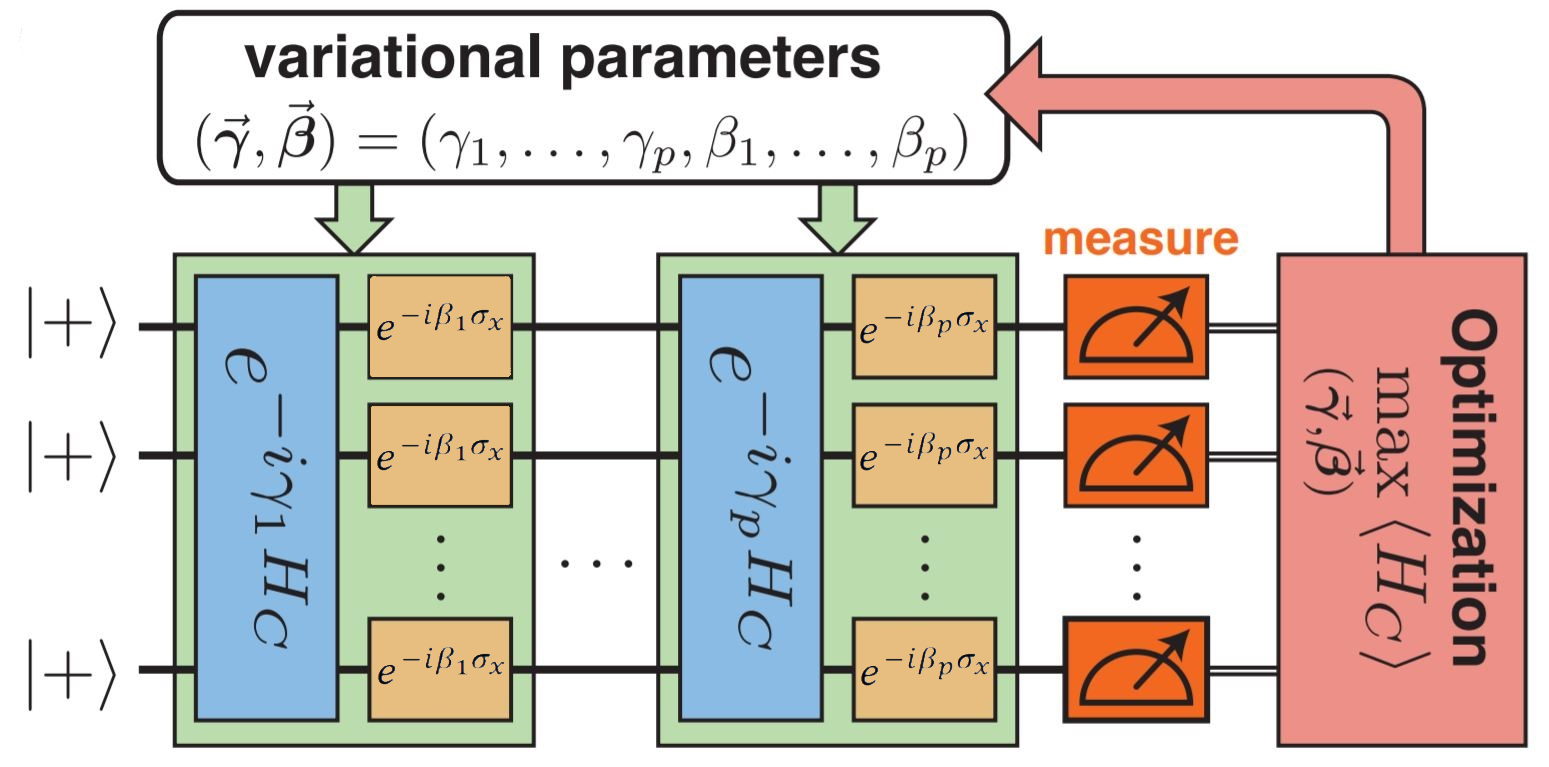
\includegraphics[width=0.7\textwidth]{figures/qaoa_idea_edit2.png}
	\caption{Schematic of a p-level Quantum Approximate Optimization Algorithm, making use of the variational approach to find optimal angles. The mixer hamiltonian is split into single qubit gates as explained in Subsection \ref{subsec:circuit}, in theory these can be applied in parallel. Adapted figure from \cite{ZWCPL18}.}
	\label{fig:schematic-qaoa-vqe}
\end{figure}

\section{Relation to the Quantum Adiabatic Algorithm}
The Quantum Adiabatic Algorithm, sometimes referred to as simply Quantum Annealing (QA), is a quantum algorithm for solving the satisfiability problem, proposed in \cite{FGGS2000} in 2000. The algorithm is based on adiabatic evolution and makes clever use of the adiabatic theorem presented in Section \ref{subsec:adiabatic-theorem}. The evolution of the quantum state is governed by the time-dependent Schr\"odinger equation
\begin{equation}
	i\frac{\partial }{\partial t} |\psi(t)\rangle = H(t)|\psi(t)\rangle
	\label{eq:schrodinger}
\end{equation}
where I included the factor $\hbar$ in $H(t)$. In QA we use a Hamiltonian $H(t)$ that interpolates between an initial Hamiltonian $H_i = H(0)$, whose ground state is easy to construct, and a final Hamiltonian $H_f = H(T)$, whose ground state encodes the satisfying assignment where $T$ is the total time of the evolution.  
\begin{equation}
H_i \xlongrightarrow{\text{time evolution}} H_f = \sum_{i=1}^m h_i
\end{equation}
Oftentimes, one uses an initial Hamiltonian $H_i$ with groundstate $|+\rangle^{\otimes n}$, which is easy to prepare on a quantum computer. A candidate for this initial Hamiltonian is $H_i = -(\sigma_x)^{\otimes n}$, with eigenvalues $1$ and $-1$ corresponding to the eigenstates $|-\rangle^{\otimes n}$ and $|+\rangle^{\otimes n}$, respectively. In the most general case we can represent the evolution using \cite{adiabatic-evolution1,adiabatic-evolution2}
\begin{equation}
H(t) = f(t)H_i + g(t)H_f
\label{eq:time-dependent hamiltonian}
\end{equation}
where $f(t)$ and g(t) are smooth functions of time with boundary conditions $f(0) = g(T) = 1$ and $f(T) = g(0) = 0$. One can simply choose a linear evolution, taking $f(t) = 1-t/T$ and $g(t) = t/T$, but other options are possible. 
Now consider the evolution of the state that is subject to this time-dependent Hamiltonian. The solution to \eqref{eq:schrodinger} defines the unitary operator $U(t,t_0)$ \cite{lecture-notes-evolution}
\begin{equation}
	|\psi(t)\rangle = U(t,t_0)|\psi(t_0)\rangle
	\label{eq:time-evolution}
\end{equation}
where $t_0$ is the initial time. Note that the operator works transitive in the sense that 
\begin{equation}
	U(t_2,t_0) = U(t_2,t_1)U(t_1,t_0)
\end{equation}
Combining \eqref{eq:schrodinger} and \eqref{eq:time-evolution}  yields the following expression
\begin{equation}
	i \frac{\partial }{\partial t} U(t,t_0)|\psi(t_0)\rangle = H(t)U(t,t_0) |\psi(t_0)\rangle
\end{equation}
and since the equation must hold for any (properly normalized) $|\psi(t)\rangle$ we find the following partial differential equation
\begin{equation}
	i \frac{\partial }{\partial t} U(t,t_0) = H(t)U(t,t_0)
	\label{eq:pde-evolution}
\end{equation}
subject to the initial condition $U(t_0,t_0) = I$ as $|\psi(t)\rangle = |\psi(t_0)\rangle$ if no time has passed.
Using a Taylor expansion and substituting the first order temporal derivative with \eqref{eq:pde-evolution} we can derive an expression for $U(t+\Delta t, t_0)$ up to second order in $\Delta t$
\begin{equation}
	U(t + \Delta t, t_0)= U(t,t_0) - i H(t)U(t,t_0)\Delta t + O(\Delta t^2)
\end{equation}
and so by using the initial condition we find
\begin{equation}
	U(t + \Delta t, t)= I - i H(t)\Delta t + O(\Delta t^2) = \exp\bigg\{-iH(t)\Delta t\bigg\} + O(\Delta t^2)
	\label{eq:taylor}
\end{equation}
where the latter equality holds because we are only concerned with terms up to $\Delta t$. Using this expression and transitivity, we can derive an expression for $U(t,t_0)$ for arbitrary timesteps $t-t_0$. We do this by dividing the time into very small steps $\epsilon = \frac{t-t_0}{N}$, so equation \eqref{eq:taylor} is approximately precise. This yield the following
\begin{equation}
	U(t,t_0) = \prod_{k=1}^N U(t_0 + k\epsilon, t_0 + (k-1)\epsilon) = \lim_{\epsilon \to 0}\prod_{k=1}^N \exp\bigg\{-i\epsilon H(t_0 + (k-1) \epsilon)\bigg\}
\end{equation}
If we can write this as an exponential of a sum, we might be able to rewrite it as an exponential of an integral when taking the limit $\epsilon \to 0$. However, we have to be wary of non-commutivity. A constant matrix always commutes with itself, but since we are considering a time-dependent matrix it might be the case that $H(t)$ does not commute with itself at different times. If $H(t_i)$ \emph{does} commute with $H(t_j)$ for every pair $t_i,t_j \in [t_0,t]$ we can write $U(t,t_0)$ as 
\begin{equation}
	U(t,t_0) = \exp \bigg\{-i\int_{t_0}^tH(t)\diff t\bigg\}, \qquad \text{ if } [H(t_i),H(t_j)] = 0 \forall t_i,t_j \in [t_0,t]
\end{equation}
Unfortunately, if $H(t_i)$ does \emph{not} commute with $H(t_j)$ for some pair $t_i,t_j \in [t_0,t]$, we need another approach. Instead, we need the \textbf{time-ordered exponential} to describe the evolution of the quantum state \cite{lecture-notes-evolution}. 

\begin{equation}
U(t,t_0) = \mathcal{T}e^{-i\int_{t_0}^t \diff \tau H(\tau)}
\end{equation}
where 
\begin{equation}
	\mathcal{T}e^{-i\int_{t_0}^t \diff \tau H(\tau)} = I + \sum_{k=1}^{\infty} \frac{(-i)^k}{k!} \int_{t_0}^t \diff t_1 \int_{t_0}^{t_1} \diff t_{2}\dots \int_{t_0}^{t_{n-1}} \diff t_n H(t_1)H(t_2)\dots H(t_n)
\end{equation}
This integral is hard to evaluate, however we can mitigate this using a the \textbf{Suzuki-Trotter} decomposition. In its most basic form we have \cite{Suzuki05}
\begin{equation}
	e^{Ax+Bx} = e^{Ax}e^{Bx} + O(x^2)
	\label{eq:suzuki-trotter}
\end{equation}
where $A$ and $B$ are arbitrary matrices and $x$ is some parameter. When applying the decomposition, one usually makes use of the relation
\begin{equation}
	\bigg(e^{\frac{x}{N}A}e^{\frac{x}{N}B}\bigg)^N = \underbrace{e^{\frac{x}{N}A}e^{\frac{x}{N}B}\dots e^{\frac{x}{N}A}e^{\frac{x}{N}B}}_{N \text{ times}} = e^{x(A+B) + \frac{1}{2}\frac{x^2}{N}[A,B] +O\big(\frac{x^3}{N^2}\big)}
\end{equation}
Note that we find $e^{(A+B)x} = (e^{\frac{x}{N}A}e^{\frac{x}{N}B})^N$ as $N$ tends to infinity. The Suzuki-Trotter expansion can be used to derive an approximation of the time-ordered exponential by discretizing the elapsed time $t-t_0$ into $N$ small intervals of length $\Delta t$ \cite{SZBW18}
\begin{equation}
	U(t,t_0) = \mathcal{T}e^{-i\int_{t_0}^t \diff \tau H(\tau)} \approx \prod_{k=0}^{N-1}\exp\bigg\{-iH(k\Delta t) \Delta t\bigg\} 
\end{equation}
Taking $H(t)$ from \eqref{eq:time-dependent hamiltonian} we have 
\begin{equation}
	\prod_{k=0}^{N-1}\exp\bigg\{-iH(k\Delta t) \Delta t\bigg\}  = \prod_{k=0}^{N-1}\exp\bigg\{-i\bigg(f(k\Delta t)H_i+ g(k\Delta t)H_f\bigg) \Delta t\bigg\}
\end{equation}
and using the approximation \eqref{eq:suzuki-trotter} we find 
\begin{equation}
	U(t,t_0) \approx \prod_{k=0}^{N-1}\exp\bigg\{-i\Delta tf(k\Delta t)H_i\bigg\}\exp\bigg\{-i\Delta t g(k\Delta t)H_f\bigg\}
\end{equation}
The approximation improves as $\Delta t$ gets smaller, and becomes exact when taking the limit $\Delta t \to 0$. Compare this with QAOA
\begin{equation}
	U_{QAOA}(\gambe) = \prod_{k=1}^p \exp\bigg\{-i\beta_k H_B\bigg\}\exp\bigg\{-i\gamma_k H_C\bigg\}
\end{equation}
 Seeing these parallels, one can consider QAOA as a discrete version of QA. Moreover, in Chapter \ref{chap:implementation} we will see that for the optimal parameter sets $\gambe$ we find that $\gamma_i$ monotonically increases and $\beta_i$ monotonically decreases, just like linear annealing in QA. These patterns were found both in \cite{ZWCPL18} and \cite{Crooks18} independently. A conceptual image of this relation is shown in Figure \ref{fig:QA-QAOA}

\begin{figure}[H]
	\centering
	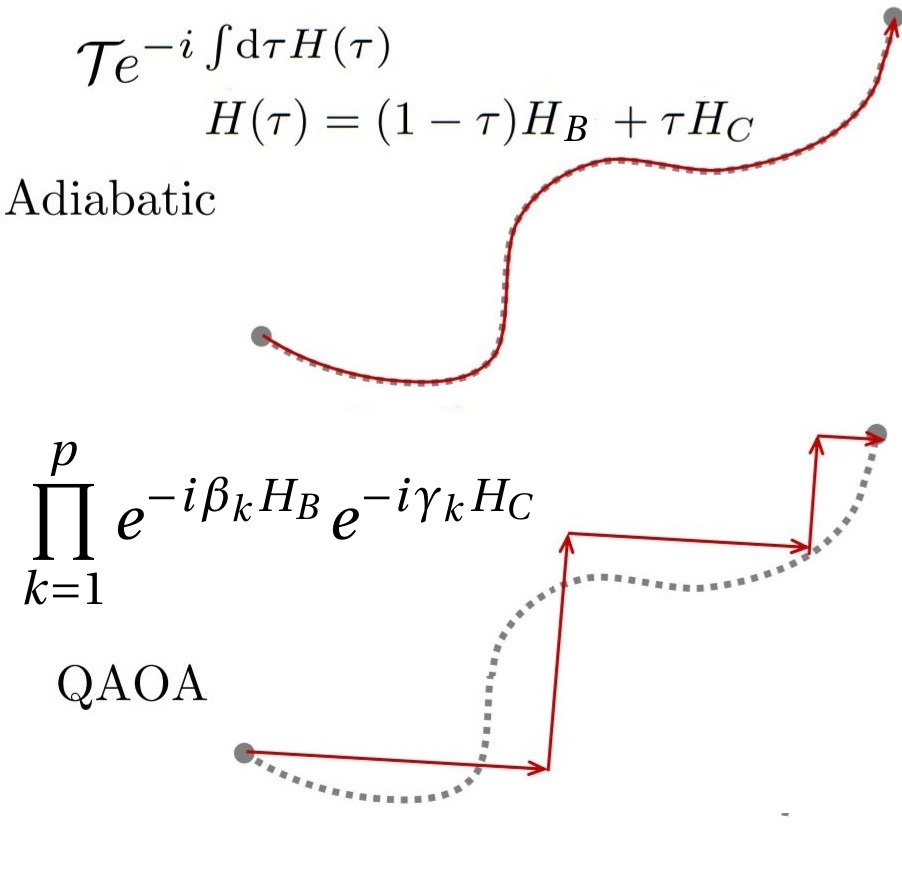
\includegraphics[width=0.4\textwidth]{figures/concept_relation_qaoa_and_qaa_edit.jpg}
	\caption{Conceptual analogy for comparing (bottom) QAOA
		to the (top) adiabatic algorithm with linear evolution as a path through state space. Adapted figure from \cite{VBB17}}
	\label{fig:QA-QAOA}
\end{figure}

In order to make sure that the system evolves to the ground state of the final Hamiltonian, the evolution must be gradual, hence the name adiabatic. Therefore, the evolution time $T$ must be long enough. It turns out that the time required for ``gradual'' evolution depends on the minimum energy gap $\Delta_{\min}$ between the groundstate and the first excited state during the evolution \cite{DMV02}.
\begin{equation}
	\Delta_{\min} \define \text{inf}\bigg\{\big|E_1(t)-E_0(t)\big|: t \in [0,T]\bigg\}
	\label{eq:spectral-gap}
\end{equation}
here $E_0(t)$ is the groundstate energy of $H(t)$, and similarly $E_1(t)$ is the energy of the first excited state. To guarantee that the system remains in the groundstate, the necessary run time of the algorithm should typically scale as $T = O(1/\Delta_{\min}^2)$ \cite{AL18, ZWCPL18}. In Figure \ref{fig:spectral-gap} an illustration of the minimum spectral gap is shown.
\begin{figure}[H]
	\centering
	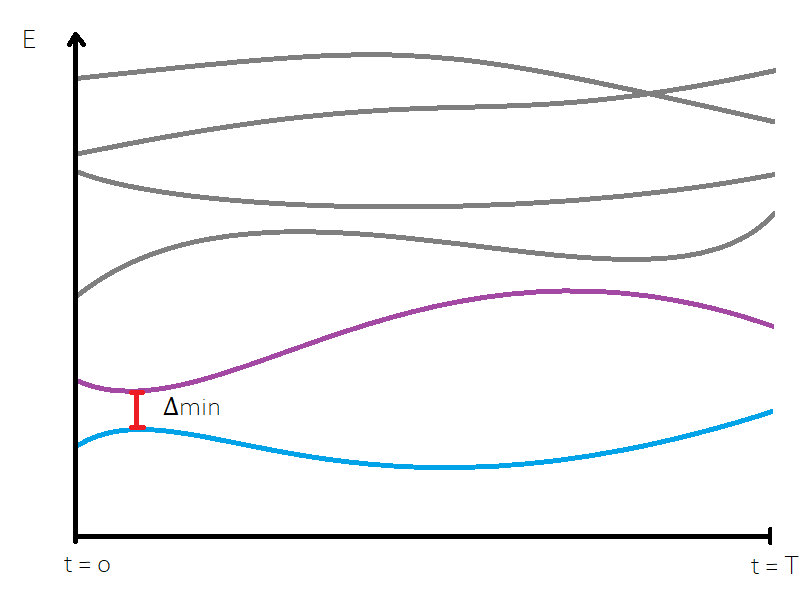
\includegraphics[width=0.5\textwidth]{figures/spectralGap.png}
	\caption{Example of an evolution of the eigenenergies of a time-dependent Hamiltonian $H(t)$. The {\color{cyan}blue} line represents the groundstate energy, and the {\color{purple}purple} line represents the energy of the first excited state. Here $\Delta_{\min}$ denotes the minimum (energy) distance between the groundstate and the first excited state of $H(t)$, as defined in \eqref{eq:spectral-gap}.}
	\label{fig:spectral-gap}
\end{figure}
A couple of years after the conception of the algorithm it turned out that for hard instances of 3SAT the gap between the lowest two energies can get exponentially close \cite{FGGN2005}. More precisely, it was shown that finding the minimum of a classical cost function whose domain is of size $N$, one needs the runtime to grow with at least the square root of $N$. In many combinatorial problems the domain size grows exponentially with the problem size $n$, so the approach is not efficient in $n$. The best one can hope for is Grover  (i.e. quadratic) speed-up, and thus the Adiabatic Algorithm does not disprove $P \neq NP$.


